\chapter{Testes}
Este capítulo tem como objetivo apresentar os testes realizados durante o desenvolvimento do projeto, que auxiliaram a fazer um controle de qualidade da aplicação com maior precisão.

% Testes Unitários
\section{Testes Unitários}
Esta seção tem como objetivo demonstrar os testes unitários realizados tanto no \textit{\gls{Back-end}} quanto no \textit{\gls{Front-end}}, que auxiliaram a validar o funcionamento desejado das funções desenvolvidas.

\subsection{Back-end}
No desenvolvimento dos testes unitários do \textit{\gls{Back-end}}, foi utilizado o pacote \textit{XUnit}, que é uma ferramenta \textit{open-source} de testes para \gls{.NET}.

A ferramenta empregada para verificar a cobertura dos testes realizados foi a \textit{Fine Code Coverage}. Na figura \ref{coverageGeralBack}, é possível observar a cobertura total dos testes na aplicação. Já a figura \ref{coverageBack} demonstra a cobertura dos testes dividida entre as camadas da aplicação.

\begin{figure}[H]
    \caption{Cobertura Geral dos testes}
	\centering
	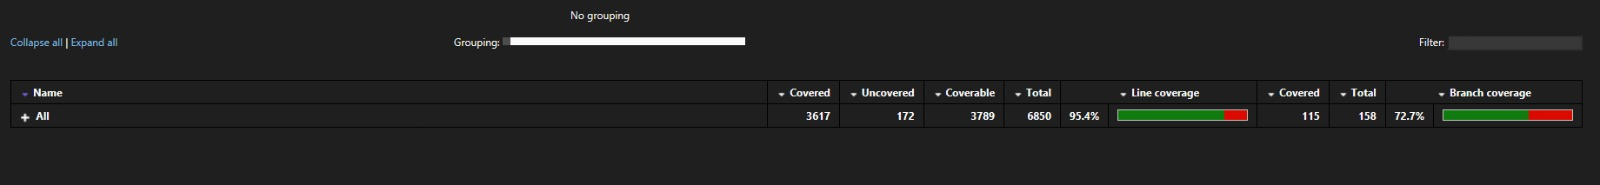
\includegraphics[width=1\textwidth]{imagens/testes/TestesUnitariosBackend/coverageGeral.jpeg}
    \label{coverageGeralBack}
	\fonte{Os autores}
\end{figure}

\begin{figure}[H]
    \caption{Cobertura dos testes por camada}
	\centering
	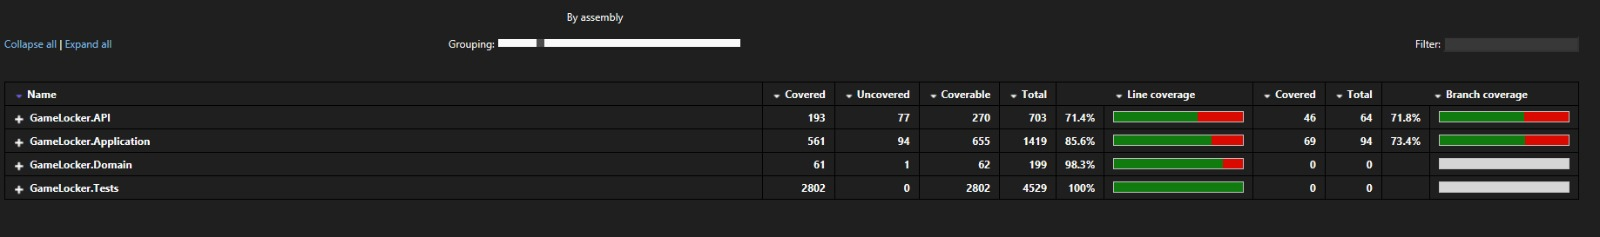
\includegraphics[width=1\textwidth]{imagens/testes/TestesUnitariosBackend/coverage.jpeg}
	\label{coverageBack}
    \fonte{Os autores}
\end{figure}
\pagebreak

A figura \ref{resultadoTestesBack} apresenta o resultado da execução dos testes, demonstrando sucesso em todos eles.

\begin{figure}[H]
    \caption{Resultado dos testes}
	\centering
	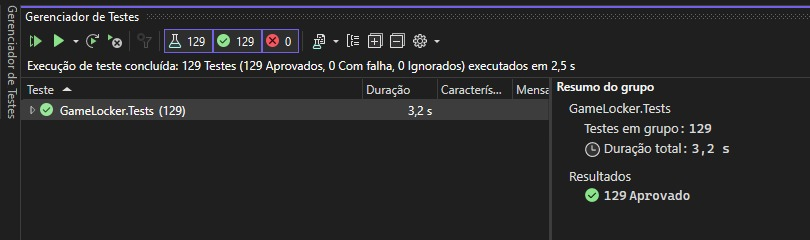
\includegraphics[width=1\textwidth]{imagens/testes/TestesUnitariosBackend/resultado.jpeg}
    \label{resultadoTestesBack}
	\fonte{Os autores}
\end{figure}

\subsection{Front-end}
Para auxiliar no desenvolvimento dos testes unitários do \textit{\gls{Front-end}}, foram utilizadas as bibliotecas \textit{Jest} e \textit{React Testing Library}.

A figura \ref{coverageFront} demonstra a cobertura de testes por página da aplicação. Já a figura \ref{coverageGeralFront} apresenta a cobertura geral, em todos os arquivos.

\begin{figure}[H]
    \caption{Cobertura dos testes por página}
	\centering
	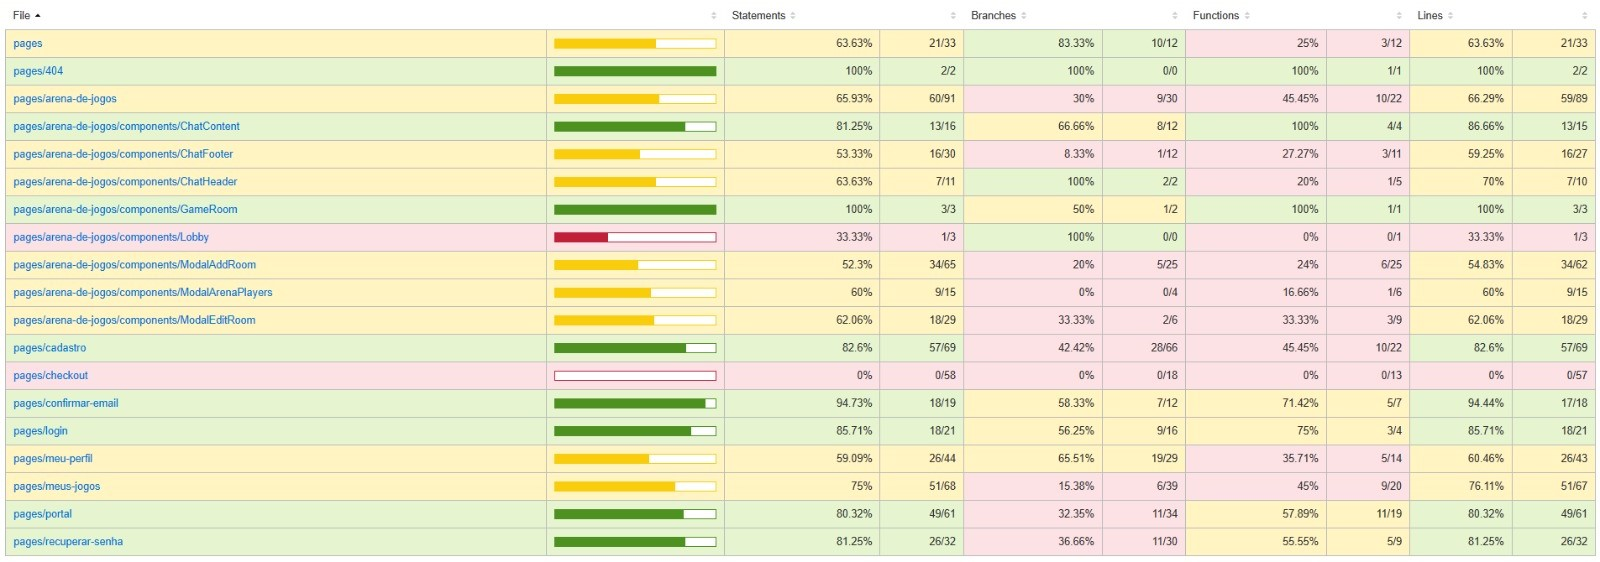
\includegraphics[width=1\textwidth]{imagens/testes/TestesUnitariosFrontend/coverageFront.jpeg}
	\label{coverageFront}
    \fonte{Os autores}
\end{figure}

\begin{figure}[H]
    \caption{Cobertura Geral dos testes}
	\centering
	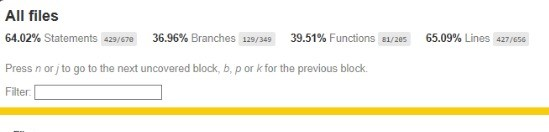
\includegraphics[width=1\textwidth]{imagens/testes/TestesUnitariosFrontend/coverageGeralFront.jpeg}
	\label{coverageGeralFront}
    \fonte{Os autores}
\end{figure}

Na figura \ref{resultadosTestesFront} é possível observar o resultado da execução dos testes, demonstrando êxito em sua totalidade.

\begin{figure}[H]
    \caption{Resultados dos testes}
	\centering
	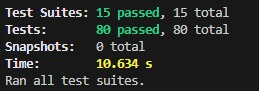
\includegraphics[width=1\textwidth]{imagens/testes/TestesUnitariosFrontend/resultadosTestesFront.jpeg}
	\label{resultadosTestesFront}
    \fonte{Os autores}
\end{figure}

% Planos de Teste
\section{Plano de Testes}

O propósito da presente seção reside na apresentação pormenorizada dos fluxos a serem adotados no âmbito dos planos de testes do sistema, tendo como desiderato a verificação da operacionalidade dos casos de uso preeminentes.

\subsubsection{Teste de Funcionalidade de Registro e Login}
\begin{enumerate}

\item{\textbf{Nome do projeto:}}
Verificando a funcionalidade de registro e login da aplicação \textit{Gamelocker};

\item{\textbf{Resumo:}}
A aplicação \textit{GameLocker} apresenta um amplo conjunto de funcionalidades. No entanto, como é comum em qualquer aplicação, é fundamental que as funções essenciais de registro e login ocorram de maneira adequada. A correta execução dessas etapas é crucial, pois permite que os usuários acessem suas contas registradas, abrindo caminho para a utilização efetiva de todas as demais funcionalidades disponíveis;

\item{\textbf{Pessoas envolvidas:}}
Os integrantes do grupo de desenvolvedores se juntaram em duplas;

\item{\textbf{Funcionalidades a serem testadas:}}
As páginas de registro e login foram selecionadas como foco dos testes das funcionalidades, visando não apenas verificar a correta execução das funções propostas, mas também avaliar a usabilidade dessas páginas;

\item{\textbf{Local dos testes:}}
Os testes serão realizados nas residências dos integrantes, em horários acordados por eles. Não tendo necessidade de se utilizar um ambiente em conjunto para tal;

\item{\textbf{Recursos necessários:}}
Os recursos necessários serão fornecidos pelos próprios testadores, que serão responsáveis por criar registros e realizar o login no site. Para facilitar o armazenamento e o acesso aos resultados de cada teste para cada membro do grupo, os testadores deverão utilizar uma ferramenta que permita o armazenamento centralizado e o acesso fácil aos dados obtidos durante o processo de testes;

\item{\textbf{Critérios usados para teste:}}
\\
\textbf{Que teste será feito:} 
\begin{itemize}
\item O teste realizado compreende uma sequência de etapas. Primeiramente, é necessário acessar a página de cadastro e preencher corretamente todas as informações requeridas, observando as diretrizes e regras estabelecidas, incluindo requisitos como tamanho mínimo de senha e escolha adequada de nome de usuário, entre outros critérios definidos. Após o preenchimento bem-sucedido do formulário de cadastro, confirmar o endereço de e-mail associado à conta. Em seguida, acessar a página de login, inserir os dados previamente cadastrados e confirmar a funcionalidade do sistema. 
\end{itemize}

\textbf{Como aplicar o teste:} 
\\
\\\textbf{Fluxo de Cadastro:}
\begin{enumerate}
\item Inserir o campo de nome;
\item Inserir o campo de sobrenome;
\item Inserir o campo de data de nascimento;
\item Inserir o campo de telefone;
\item Inserir o campo de nome de usuário;
\item Caso haja algum campo incorreto durante o processo de registro ou login, exibir mensagens de erro específicas no modal correspondente;
\item Com todos os campos preenchidos corretamente, o botão de continuar o cadastro estará habilitado;
\item Clicar no botão continuar;
\item Inserir o campo de e-mail;
\item Inserir a campo de senha;
\item Preencher o campo de confirmar senha;
\item Clicar no botão de cadastrar;
\item Caso haja algum campo incorreto durante o processo de registro ou login, exibir mensagens de erro específicas no modal correspondente;
\item Se todas as informações estiverem corretamente preenchidas pelo usuário, será solicitada a confirmação do endereço de e-mail.
\item Após a confirmação, um modal será exibido, informando que o cadastro foi realizado com sucesso.
\item Em seguida, o sistema redirecionará o usuário para a tela de login, onde ele poderá realizar o acesso à sua conta.
\end{enumerate}

\textbf{Fluxo de Login:}
\begin{enumerate}
\item Inserir o campo de e-mail;
\item Inserir o campo de senha;
\item Clicar no botão de ``Entrar'', caso algum dos campos preenchidos esteja em desacordo com as informações fornecidas durante o cadastro, o usuário deverá ser prontamente notificado;
\item Caso os campos estejam corretamente preenchidos, o usuário será redirecionado para a tela de portal.
\end{enumerate}

\item{\textbf{Riscos:}}
\begin{itemize}
\item No caso de algum dos testadores não conseguir realizar suas atividades, é imprescindível que os demais sejam informados para que seja feita uma organização adequada e garantir que todas as etapas de teste sejam concluídas;
\item Devido a problemas de hospedagem, ocorrer uma falta de conexão com o \textit{\gls{Back-end}}, exigindo a realização de testes em ambiente local.
\end{itemize}

\item{\textbf{Como os resultados do teste serão divulgados:}}
Ao final desta seção de planejamento dos testes, encontra-se um quadro que indica o resultado de cada um dos testes realizados, classificando-os como sucesso ou falha. Caso ocorra uma falha, será apresentada a motivação subjacente a ela.
\end{enumerate}

\subsubsection{Teste de Funcionalidade do Sistema de Reviews}
\begin{enumerate}

\item{\textbf{Nome do projeto:}}
Verificando a funcionalidade do sistema de reviews;

\item{\textbf{Resumo:}}
A funcionalidade central do site \textit{GameLocker} baseia-se em avaliações. Portanto, é necessário que essa funcionalidade funcione corretamente, a fim de garantir que o site cumpra o que se propôs a realizar;

\item{\textbf{Pessoas envolvidas:}}
Os integrantes do grupo de desenvolvedores se juntaram em duplas;

\item{\textbf{Funcionalidades a serem testadas:}}
Todas as funções relacionadas às avaliações foram submetidas a testes (Criação, Visualização, Edição e Exclusão) a fim de garantir uma usabilidade correta da proposição do site;

\item{\textbf{Local dos testes:}}
Os testes serão realizados nas residências dos integrantes, em horários acordados por eles. Não tendo necessidade de se utilizar um ambiente em conjunto para tal;

\item{\textbf{Recursos necessários:}}
Os recursos necessários serão fornecidos pelos próprios testadores, que serão responsáveis por criar registros e realizar o login no site. Para facilitar o armazenamento e o acesso aos resultados de cada teste para cada membro do grupo, os testadores deverão utilizar uma ferramenta que permita o armazenamento centralizado e o acesso fácil aos dados obtidos durante o processo de testes;

\item{\textbf{Critérios usados para teste:}}
\\
\textbf{Que teste será feito:} 
\begin{itemize}
\item Criação de uma review para um jogo específico escolhido pelo usuário, adicionando todos os dados necessários;
\item Visualização dessa revisão na tela de perfil de usuário;
\item Edição dessa review, atualizando na tela de perfil;
\item Remoção dessa revisão, a excluindo.
\end{itemize}

\textbf{Como aplicar o teste:} 
\\
\textbf{Fluxo de Criação:}
\begin{enumerate}
\item Escolher o jogo no qual será feita a review;
\item Inserir um comentário sobre esse jogo;
\item Inserir uma nota de 0 a 10;
\item Inserir o status do jogo (Jogando, Dropado, Zerado, Desejado);
\item Finalizar a review;
\item Com tudo ocorrendo da maneira correta, a review terá sido adicionada ao perfil do usuário.
\end{enumerate}

\textbf{Fluxo de Visualização:}
\begin{enumerate}
\item Entrar na tela de meu perfil;
\item Buscar qual review é desejado para visualização;
\item Clicar na review e visualizar os comentários, status e nota dada.
\end{enumerate}

\textbf{Fluxo de Edição:}
\begin{enumerate}
\item Entrar na tela de meu perfil;
\item Buscar qual review é desejado para edição;
\item Clicar na review e visualizá-la por completo;
\item Alterar os campos desejados, tais como mudar a nota de 6 para 10;
\item Salvar as alterações;
\item Fechar o modal de review.
\end{enumerate}

\textbf{Fluxo de Exclusão:}
\begin{enumerate}
\item Entrar na tela de meu perfil;
\item Buscar qual review é desejado para remoção;
\item Clicar na review e visualizá-la por completo;
\item Selecionar a opção de excluir.
\end{enumerate}

\item{\textbf{Riscos:}}
\begin{itemize}
\item No caso de algum dos testadores não conseguir realizar suas atividades, é imprescindível que os demais sejam informados para que seja feita uma organização adequada e garantir que todas as etapas de teste sejam concluídas;
\item Devido a problemas de hospedagem, ocorrer uma falta de conexão com o \textit{\gls{Back-end}}, exigindo a realização de testes em ambiente local.
\end{itemize}

\item{\textbf{Como os resultados dos testes serão divulgados:}}
Ao final desta seção de planejamento dos testes, encontra-se um quadro que indica o resultado de cada um dos testes realizados, classificando-os como sucesso ou falha. Caso ocorra uma falha, será apresentada a motivação subjacente a ela.
\end{enumerate}

\subsubsection{Teste de Funcionalidade de Pagamento de Assinatura}

\begin{enumerate}

\item{\textbf{Nome do projeto:}}
Testando a Funcionalidade de Pagamento de Assinatura da aplicação \textit{Gamelocker};

\item{\textbf{Resumo:}}
O teste tem como objetivo verificar a funcionalidade do sistema de pagamento de assinatura do \textit{GameLocker}, garantindo que os usuários possam se inscrever, fornecer informações de pagamento corretas e segura, e ter acesso aos serviços premium após o pagamento;

\item{\textbf{Pessoas envolvidas:}}
Os integrantes do grupo de desenvolvedores se juntaram em duplas;

\item{\textbf{Funcionalidades a serem testadas:}}
Na página de inscrição do sistema, garantir que o formulário de inscrição esteja completo e funcional, permitindo aos usuários escolher o tipo de assinatura desejada. Em relação ao processo de pagamento, testar o funcionamento da integração com a \gls{api} do \gls{MercadoPago}, enquanto se verifica rigorosamente se os detalhes do cartão são criptografados e protegidos para assegurar a segurança dos dados. Além disso, após o pagamento bem-sucedido, confirmar se os usuários recebem uma confirmação, proporcionando uma garantia adicional da transação, e se eles têm acesso imediato aos recursos premium, demonstrando a eficiência do processo de ativação;

\item{\textbf{Local dos testes:}}
Os testes serão realizados nas residências dos integrantes, em horários acordados por eles. Não tendo necessidade de se utilizar um ambiente em conjunto para tal;

\item{\textbf{Recursos necessários:}}
Um ambiente de testes isolado do ambiente de produção, evitando transações reais. Para simular cenários diversos, utilizar cartões de crédito de teste fornecidos pelo provedor do gateway e explorar emuladores de pagamento. O acesso à documentação técnica completa do gateway, incluindo informações sobre endpoints de API, formatos de dados, códigos de erro e exemplos de solicitações e respostas. Além disso, um ambiente de teste para o sistema, permitindo simular interações de usuários, implementar registros detalhados no sistema, rastreando todas as interações com o gateway de pagamento, para diagnosticar falhas durante os testes;

\item{\textbf{Critérios usados para teste:}}
\\
\textbf{Que teste será feito:} 
\begin{itemize}
\item Inserção dos dados no formulário de assinatura, incluindo uma verificação da integridade dos dados inseridos;
\item Testes rigorosos para as funcionalidades antifraude do gateway. Isso inclui verificações detalhadas do CVV, visando identificar e bloquear transações fraudulentas;
\item Simular diferentes cenários de pagamento para testar a eficácia do sistema. Isso envolve a realização de testes para transações bem-sucedidas, identificação de falhas no pagamento e processos de reembolso.
\item Verificar o acesso imediato aos recursos disponíveis aos usuários \textit{premiums};
\end{itemize}

\item{\textbf{Riscos:}}
\begin{itemize}
\item No caso de algum dos testadores não conseguir realizar suas atividades, é imprescindível que os demais sejam informados para que seja feita uma organização adequada e garantir que todas as etapas de teste sejam concluídas;
\item Problemas de processamento de pagamento que podem atrasar o acesso dos usuários aos serviços premium;
\item Erros de segurança que podem comprometer as informações de pagamento dos usuários.
\end{itemize}

\item{\textbf{Como os resultados do teste serão divulgados:}}
Ao final desta seção de planejamento dos testes, encontra-se um quadro que indica o resultado de cada um dos testes realizados, classificando-os como sucesso ou falha. Caso ocorra uma falha, será apresentada a motivação subjacente a ela.
\end{enumerate}

\subsubsection{Teste de Funcionalidade da Arena de Jogos}
\begin{enumerate}

\item{\textbf{Nome do projeto:}}
Verificando a funcionalidade da Arena de Jogos da aplicação \textit{Gamelocker};

\item{\textbf{Resumo:}}
O teste visa verificar a funcionalidade das Arenas de Jogos no \textit{GameLocker}. Isto inclui garantir que os usuários possam criar salas, configurar regras de jogos e se comunicar por meio de chats. Além disso, será verificado se os administradores têm controle efetivo sobre as salas e se os jogadores podem participar e interagir de forma adequada;

\item{\textbf{Pessoas envolvidas:}}
Os integrantes do grupo de desenvolvedores se juntaram em duplas;

\item{\textbf{Funcionalidades a serem testadas:}}
\begin{itemize}
\item Verificar se os usuários podem criar salas, especificar o tipo de jogo, o número de jogadores e outras configurações relevantes;
\item Garantir que cada sala tenha um chat funcional para permitir a comunicação entre os jogadores durante o jogo;
\item Verificar se os administradores têm controle efetivo sobre a sala, podendo modificar as configurações da sala conforme necessário.
\item Verificar se apenas usuários premium podem criar salas.
\end{itemize}

\item{\textbf{Local dos testes:}}
Os testes serão realizados nas residências dos integrantes, em horários acordados por eles. Não tendo necessidade de se utilizar um ambiente em conjunto para tal;

\item{\textbf{Recursos necessários:}}
Os recursos necessários serão fornecidos pelos próprios testadores, que serão responsáveis por criar registros e realizar o login no site. Para facilitar o armazenamento e o acesso aos resultados de cada teste para cada membro do grupo, os testadores deverão utilizar uma ferramenta que permita o armazenamento centralizado e o acesso fácil aos dados obtidos durante o processo de testes;

\item{\textbf{Critérios usados para teste:}}
\\
\textbf{Que teste será feito:} 
\begin{itemize}
\item Verificar se os usuários premium podem criar salas com sucesso;
\item Testar a implementação do chat, incluindo a capacidade de enviar mensagens e \textit{emojis};
\item Avaliar se os administradores têm controle total sobre as configurações da sala.
\end{itemize}

\item{\textbf{Riscos:}}
\begin{itemize}
\item No caso de algum dos testadores não conseguir realizar suas atividades, é imprescindível que os demais sejam informados para que seja feita uma organização adequada e garantir que todas as etapas de teste sejam concluídas;
\item Devido a problemas de hospedagem, ocorrer uma falta de conexão com o \textit{\gls{Back-end}}, exigindo a realização de testes em ambiente local.
\end{itemize}

\item{\textbf{Como os resultados do teste serão divulgados:}}
Ao final desta seção de planejamento dos testes, encontra-se um quadro que indica o resultado de cada um dos testes realizados, classificando-os como sucesso ou falha. Caso ocorra uma falha, será apresentada a motivação subjacente a ela.
\end{enumerate}

\subsubsection{Quadro de resultados dos testes}
\begin{quadro}[H]
\centering
\caption{Resultados dos Testes}
\label{tab:resultadoteste}
\begin{longtable}{|p{10cm}|p{3cm}|}
\hline
\centering Teste & \centering Resultado
\hline
Funcionalidade de Registro e Login & Sucesso
\\\hline
Funcionalidade do Sistema de Reviews & Sucesso
\\\hline
Funcionalidade de Pagamento de Assinatura & Sucesso
\\\hline
Funcionalidade da Arena de Jogos & Sucesso
\\\hline
\end{longtable}
\fonte{Os Autores.}
\end{quadro}

\section{Testes de Segurança}
Esta seção demonstra os testes de segurança nos quais a aplicação deve ser aprovada, de acordo com as regras da disciplina, buscando garantir uma maior proteção do sistema.

\subsection{Teste de SSL}
Foi utilizada a plataforma SSL Labs \url{https://www.ssllabs.com/ssltest/} para realização deste teste.

Na figura \ref{testeSSL}, é possível observar que a aplicação GameLocker recebeu nota A+ na verificação realizada, demonstrando uma forte segurança na comunicação entre o domínio do site e os navegadores, de forma criptografada.

\begin{figure}[H]
        \center
	\caption{\label{fig_sge20}Resultado do teste de SSL}
    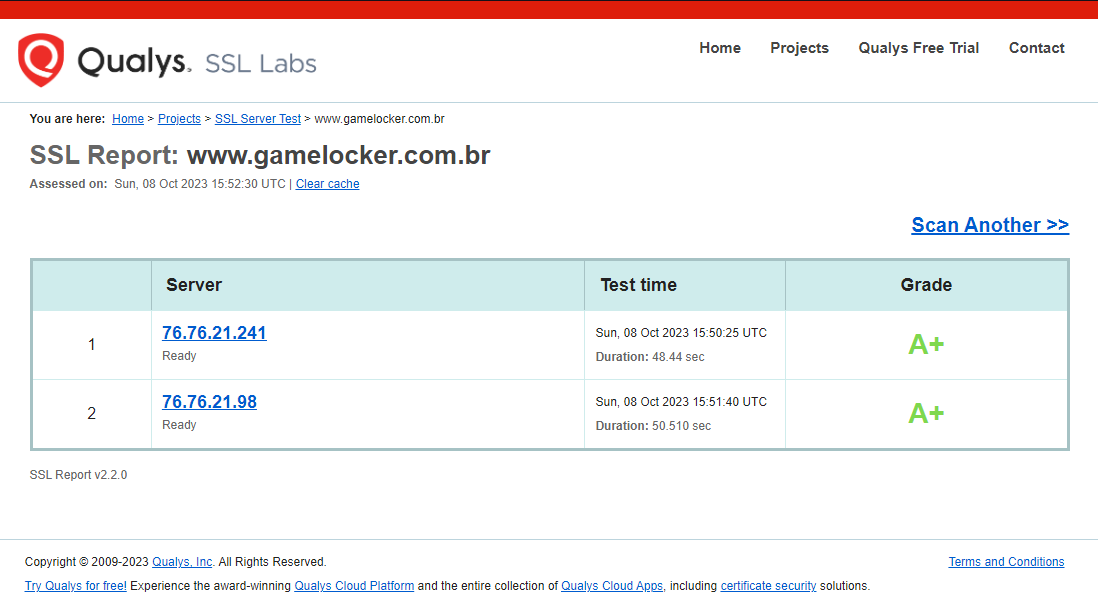
\includegraphics[scale=0.50]{imagens/testes/TESTESSL.png}
    \label{testeSSL}
	\fonte{Os autores}
\end{figure}

\subsection{Teste de Headers}
Este teste tem como objetivo verificar a segurança dos \gls{Headers} nas requisições \ac{https} realizadas pela aplicação. Para isso, foi utilizada a plataforma Security Headers, disponível em: \url{securityheaders.io}

A figura \ref{testeHeaders} apresenta o resultado do teste realizado, indicando um nível satisfatório de segurança nos \gls{Headers} utilizados na aplicação.

\begin{figure}[H]
    \center
	\caption{\label{fig_sge20}Resultado do teste de Headers}
    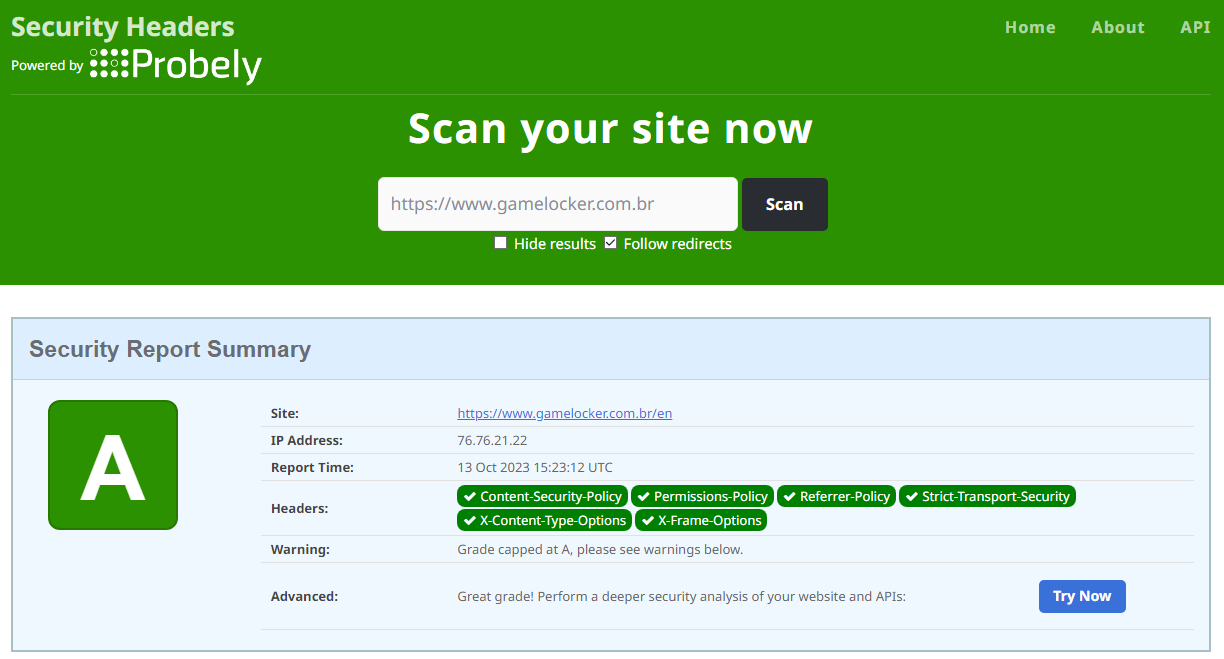
\includegraphics[scale=0.45]{imagens/testes/TESTEHEADERS.png}
    \label{testeHeaders}
	\fonte{Os autores}
\end{figure}